\documentclass[12pt,letterpaper]{article}
\usepackage{graphicx,textcomp}
\usepackage{natbib}
\usepackage{setspace}
\usepackage{fullpage}
\usepackage{color}
\usepackage[reqno]{amsmath}
\usepackage{amsthm}
\usepackage{fancyvrb}
\usepackage{amssymb,enumerate}
\usepackage[all]{xy}
\usepackage{endnotes}
\usepackage{lscape}
\newtheorem{com}{Comment}
\usepackage{float}
\usepackage{hyperref}
\newtheorem{lem} {Lemma}
\newtheorem{prop}{Proposition}
\newtheorem{thm}{Theorem}
\newtheorem{defn}{Definition}
\newtheorem{cor}{Corollary}
\newtheorem{obs}{Observation}
\usepackage[compact]{titlesec}
\usepackage{dcolumn}
\usepackage{tikz}
\usetikzlibrary{arrows}
\usepackage{multirow}
\usepackage{xcolor}
\newcolumntype{.}{D{.}{.}{-1}}
\newcolumntype{d}[1]{D{.}{.}{#1}}
\definecolor{light-gray}{gray}{0.65}
\usepackage{url}
\usepackage{listings}
\usepackage{color}

\definecolor{codegreen}{rgb}{0,0.6,0}
\definecolor{codegray}{rgb}{0.5,0.5,0.5}
\definecolor{codepurple}{rgb}{0.58,0,0.82}
\definecolor{backcolour}{rgb}{0.95,0.95,0.92}

\lstdefinestyle{mystyle}{
	backgroundcolor=\color{backcolour},   
	commentstyle=\color{codegreen},
	keywordstyle=\color{magenta},
	numberstyle=\tiny\color{codegray},
	stringstyle=\color{codepurple},
	basicstyle=\footnotesize,
	breakatwhitespace=false,         
	breaklines=true,                 
	captionpos=b,                    
	keepspaces=true,                 
	numbers=left,                    
	numbersep=5pt,                  
	showspaces=false,                
	showstringspaces=false,
	showtabs=false,                  
	tabsize=2
}
\lstset{style=mystyle}
\newcommand{\Sref}[1]{Section~\ref{#1}}
\newtheorem{hyp}{Hypothesis}

\title{Problem Set 1}
\date{Due: September 30, 2024}
\author{Applied Stats/Quant Methods 1}

\begin{document}
	\maketitle
	
	\section*{Instructions}
	\begin{itemize}
	\item Please show your work! You may lose points by simply writing in the answer. If the problem requires you to execute commands in \texttt{R}, please include the code you used to get your answers. Please also include the \texttt{.R} file that contains your code. If you are not sure if work needs to be shown for a particular problem, please ask.
\item Your homework should be submitted electronically on GitHub.
\item This problem set is due before 23:59 on Monday September 30, 2024. No late assignments will be accepted.
%\item Total available points for this homework is 80.
	\end{itemize}
	
	\vspace{1cm}
	\section*{Question 1: Education}

A school counselor was curious about the average of IQ of the students in her school and took a random sample of 25 students' IQ scores. The following is the data set:\\
\vspace{.5cm}

\lstinputlisting[language=R, firstline=36, lastline=36]{PS01_ZexiWang.R}  

\vspace{1cm}

\begin{enumerate}
	\item Find a 90\% confidence interval for the average student IQ in the school.\\
	\lstinputlisting[language=R, firstline=36, lastline=49]{PS01_ZexiWang.R} 
\noindent Answer: 90\% confidence interval for the average student IQ in the school is: ( 94.15 , 102.73 )

	\item Next, the school counselor was curious  whether  the average student IQ in her school is higher than the average IQ score (100) among all the schools in the country.\\ 
	
	\noindent Using the same sample, conduct the appropriate hypothesis test with $\alpha=0.05$.
	\lstinputlisting[language=R, firstline=51, lastline=53]{PS01_ZexiWang.R} 
\noindent Answer: t-test results indicate that the average student IQ in this school is not significantly different from the average IQ score of 100 among all schools in the country( p = 0.5569 \textgreater 0.05)
\end{enumerate}

\newpage

	\section*{Question 2: Political Economy}

\noindent Researchers are curious about what affects the amount of money communities spend on addressing homelessness. The following variables constitute our data set about social welfare expenditures in the USA. \\
\vspace{.5cm}


\begin{tabular}{r|l}
	\texttt{State} &\emph{50 states in US} \\
	\texttt{Y} & \emph{per capita expenditure on shelters/housing assistance in state}\\
	\texttt{X1} &\emph{per capita personal income in state} \\
	\texttt{X2} &  \emph{Number of residents per 100,000 that are "financially insecure" in state}\\
	\texttt{X3} &  \emph{Number of people per thousand residing in urban areas in state} \\
	\texttt{Region} &  \emph{1=Northeast, 2= North Central, 3= South, 4=West} \\
\end{tabular}

\vspace{.5cm}
\noindent Explore the \texttt{expenditure} data set and import data into \texttt{R}.

\lstinputlisting[language=R, firstline=54, lastline=54]{PS01_ZexiWang.R}  

\begin{itemize}

\lstinputlisting[language=R, firstline=59, lastline=59]{PS01_ZexiWang.R}  
\item
Please plot the relationships among \emph{Y}, \emph{X1}, \emph{X2}, and \emph{X3}? What are the correlations among them (you just need to describe the graph and the relationships among them)?
\lstinputlisting[language=R, firstline=61, lastline=95]{PS01_ZexiWang.R}  
\begin{figure}[H]
	\centering
	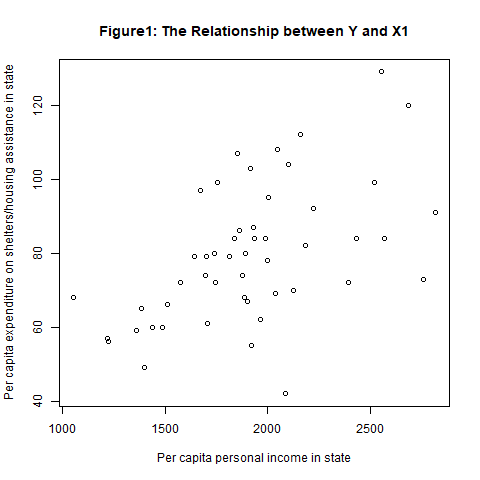
\includegraphics[width=.55\textwidth]{Y~X1.png}
\end{figure}
\noindent The correlation coefficient between Y and X1 is 0.531, Figure 1 illustrates that as X1 increases, the value of Y also increases gradually. \\

\begin{figure}[H]
	\centering
	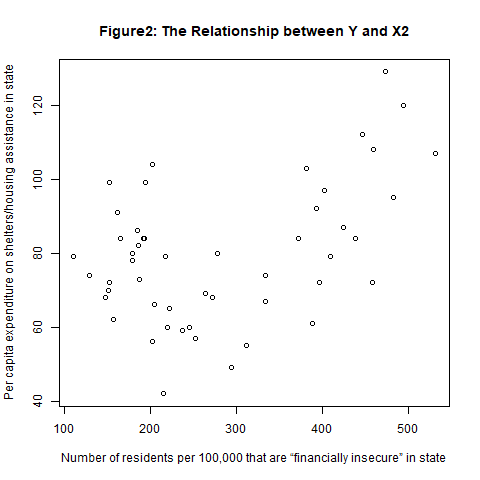
\includegraphics[width=.55\textwidth]{Y~X2.png}
\end{figure}
\noindent The correlation coefficient between Y and X2 is 0.448, Figure 2 illustrates that as X2 increases, Y decreases until X2 reaches approximately 300, at which point Y begins to increase with further increases in X2. \\

\begin{figure}[H]
	\centering
	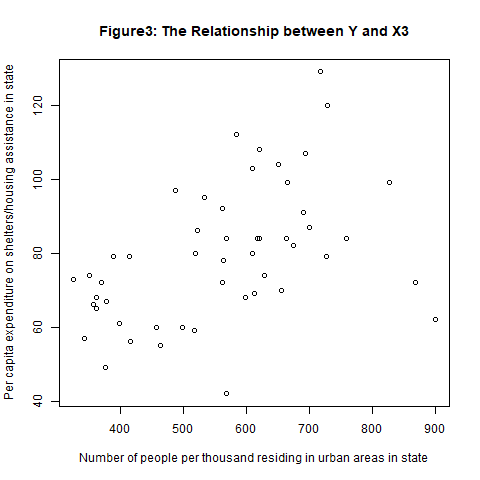
\includegraphics[width=.55\textwidth]{Y~X3.png}
\end{figure}
\noindent The correlation coefficient between Y and X3 is 0.463, Figure 3 illustrates that as X3 increases, the value of Y also increases gradually. \\

\lstinputlisting[language=R, firstline=96, lastline=126]{PS01_ZexiWang.R}  

\begin{figure}[H]
	\centering
	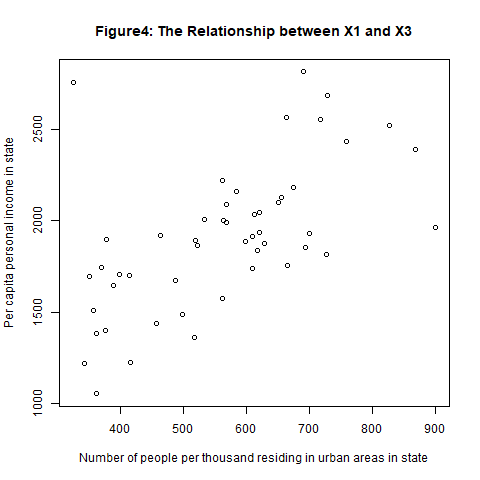
\includegraphics[width=.55\textwidth]{X1~X3.png}
\end{figure}
\noindent The correlation coefficient between Y and X3 is 0.595, Figure4 demonstrate that as X3 increase, X1 also rises correspondingly. \\

\begin{figure}[H]
	\centering
	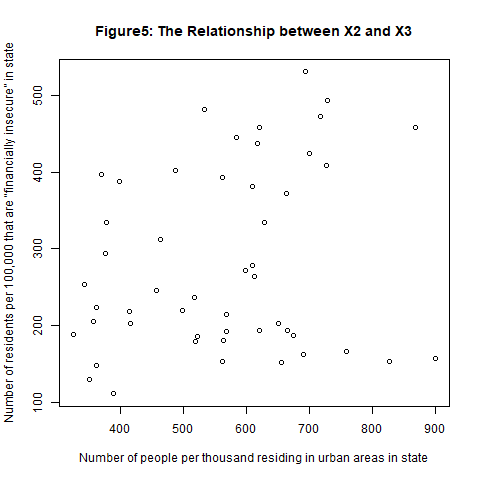
\includegraphics[width=.55\textwidth]{X2~X3.png}
\end{figure}
\noindent The correlation coefficient between Y and X3 is 0.463, Figure 3 illustrates that as X3 increases, the value of Y also increases gradually. \\

\begin{figure}[H]
	\centering
	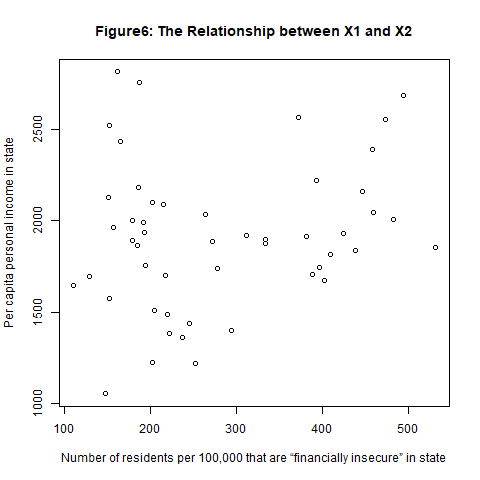
\includegraphics[width=.55\textwidth]{X1~X2.png}
\end{figure}
\noindent The correlation coefficient between Y and X3 is 0.463, Figure 3 illustrates that as X3 increases, the value of Y also increases gradually. \\

\item
Please plot the relationship between \emph{Y} and \emph{Region}? On average, which region has the highest per capita expenditure on housing assistance?
\lstinputlisting[language=R, firstline=129, lastline=137]{PS01_ZexiWang.R}
\begin{figure}[H]
	\centering
	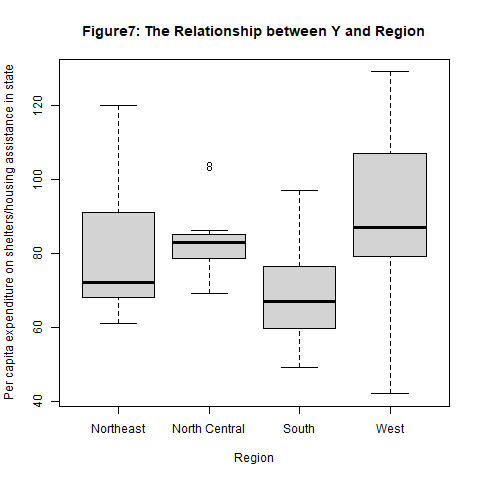
\includegraphics[width=.55\textwidth]{Y~Region.png}
\end{figure}
\noindent The box plot (Figure7) indicates that West Region (Region 4) has the highest per capita expenditure on housing assistance. \\

\item
Please plot the relationship between \emph{Y} and \emph{X1}? Describe this graph and the relationship. Reproduce the above graph including one more variable \emph{Region} and display different regions with different types of symbols and colors.
\lstinputlisting[language=R, firstline=139, lastline=162]{PS01_ZexiWang.R} 
\begin{figure}[H]
	\centering
	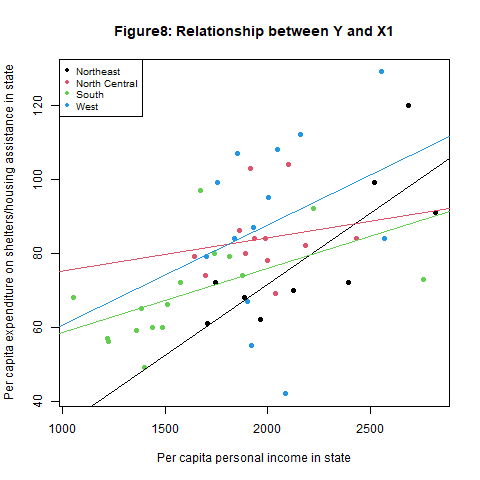
\includegraphics[width=.6\textwidth]{Y~X1_Region.png}
\end{figure} 
\noindent Figure8 indicates that as per capita personal income increases, the per capita expenditure on housing assistance also increases accordingly. This suggests that states with higher economic development and per capita income may be more inclined to invest more funds in housing assistance. \\

\end{itemize}
\end{document}
